\documentclass[11pt]{report}
% Basic Packages for Encoding (Input AND Output) and Langauge Support
\usepackage[utf8]{inputenc}
\usepackage[T1]{fontenc}
\usepackage[french, english]{babel}
\usepackage{lmodern}

% Importer un document externe 
% Utiliser \import{directory}{file}
\usepackage{import}

% Change Layout with a User-Friendly Interface
\usepackage[margin=1in]{geometry}

% Include Pictures with a User-Friendly Interface
\usepackage{graphicx}
\usepackage{float}

% Extended Math Support from the Famous 'American Mathematical Society'
\usepackage{amsmath}
\usepackage{amsfonts}
\usepackage{amssymb}

% Just for Demonstration Purposes
\usepackage[math]{blindtext}

% For use on computer
\usepackage{hyperref}

% For table color
\usepackage{xcolor,colortbl}

% Tableau verticale
\usepackage{rotating}

% Figure dans figure
\usepackage{subfig}

% Multicolumn
\usepackage{multirow}

% Preuves
\usepackage{amsthm}

% Bibliographie
\usepackage[backend=bibtex,style=trad-plain]{biblatex} %Imports biblatex package
\addbibresource{sources.bib} %Import the bibliography file

% Page style
\usepackage{fancyhdr}

\fancyhead{} % clear all header fields
\fancyhead[L]{\textbf{Les algorithmes quantiques}}
\fancyhead[R]{\textit{\nouppercase{\leftmark}}}
\fancyfoot{} % clear all footer fields
\fancyfoot[R]{\thepage}
\fancyfoot[L]{Romain Blondel}

% Title settings
\setlength{\parindent}{0cm}
\setlength{\parskip}{1ex plus 0.5ex minus 0.2ex}
\newcommand{\hsp}{\hspace{20pt}}
\newcommand{\HRule}{\rule{\linewidth}{0.5mm}}

% Dummy text
\usepackage{lipsum} 

% Titre
\usepackage[affil-it]{authblk}
\title{\textbf{Les algorithmes quantiques} \\ \textit{Ou une théorie de recherche}}
\author{Romain Blondel}
\affil{Gymnase Auguste Piccard}

% Page num
\renewcommand{\thepage}{}

\begin{document}
\selectlanguage{french}

% Page de garde
\begin{titlepage}
  \begin{sffamily}
  \begin{center}

    \textsc{\LARGE Gymnase Auguste Piccard}\\[2cm]

    \textsc{\Large Travail de maturité}\\[1.5cm]

    \HRule \\[0.4cm]
    { \huge \textbf{Les algorithmes quantiques} \\ \textit{Ou une théorie d'optimisation} \\[0.4cm] }

    \HRule \\[2cm]
    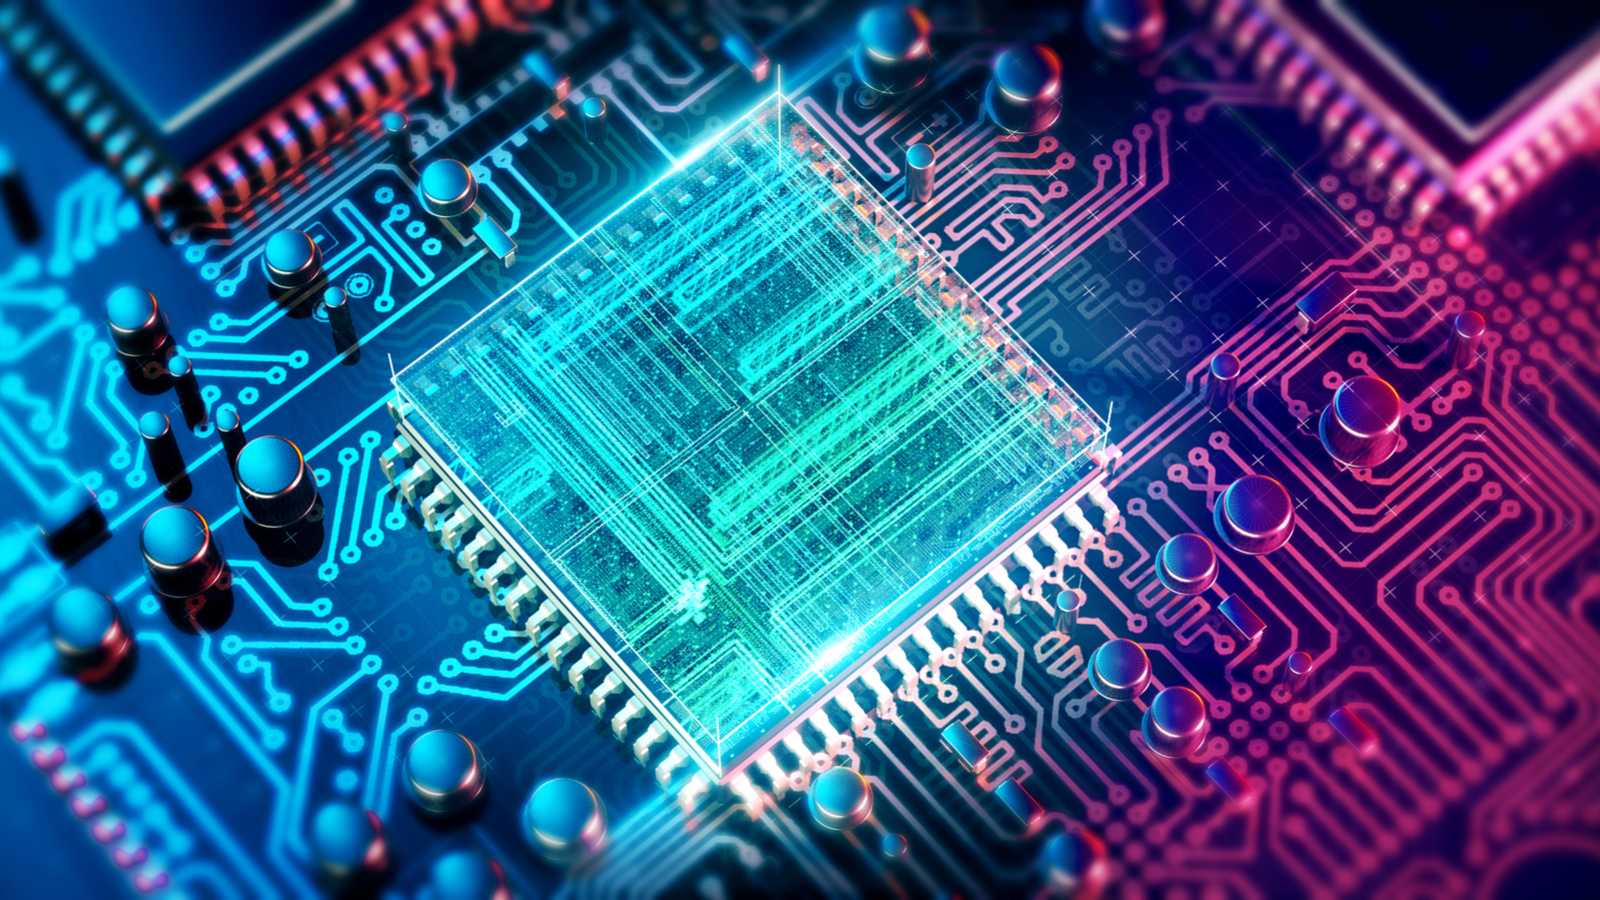
\includegraphics[scale=0.2]{Images/illustration.jpg}
    \\[2cm]

	\vspace*{\fill}

    \begin{minipage}{0.3\textwidth}
      \begin{flushleft} \large
        Romain \textsc{Blondel}\\
      \end{flushleft}
    \end{minipage}
    \begin{minipage}{0.3\textwidth}
      \centering
      \today
    \end{minipage}
    \begin{minipage}{0.3\textwidth}
      \begin{flushright} \large
        \emph{Classe :} \textsc{2M8}\\
      \end{flushright}
    \end{minipage}

  \end{center}
  \end{sffamily}
\end{titlepage}

% Abstract
\selectlanguage{english}
\begin{abstract}
\selectlanguage{french}

\lipsum[1-1]

\end{abstract}
\selectlanguage{french}
\clearpage

% Table des matieres

% Page num
\renewcommand{\thepage}{\arabic{page}}
\setcounter{page}{1}
\pagestyle{fancy}

\tableofcontents
\clearpage

% Texte
\part{Préambules}
\chapter{Introduction}
\lipsum[2-4]

\chapter{Notions théoriques}
\section{Informatique}
\lipsum[2-4]

\section{Physique}
\lipsum[2-4]

\part{Les notions de base}
\chapter{Un ordinateur classique}
\section{Logique}
\lipsum[2-4]
\section{Hardware}
\lipsum[2-4]

\chapter{Un qubit}
\section{Superposition d'états}
\lipsum[2-4]

\section{Opérations sur un qubit}
\lipsum[2-4]

\section{Mesure}
\lipsum[2-4]

\chapter{Système à plusieurs qubits}
\section{Description du système}
\lipsum[2-4]

\section{Les portes}
\lipsum[2-4]

\section{Superposition}
\lipsum[2-4]

\subsection{Superdense Coding}
\lipsum[2-4]

\subsection{Quantum Teleportation}
\lipsum[2-4]

\part{Exemples d'algorithmes}
\chapter{Algorithme de Deutsch-Jozsa}
\lipsum[2-4]

\chapter{Quelques protocoles}
\lipsum[2-4]

\section{Phase kickback}
\lipsum[2-4]

\section{Quantum Fourier Transform}
\lipsum[2-4]

\section{Quantum Phase Estimation}
\lipsum[2-4]

\chapter{Algorithme de Shor}
\lipsum[2-4]

\section{Principe}
\lipsum[2-4]

\section{Implémentation simple}
\lipsum[2-4]

\subsection{Simulation}
\lipsum[2-4]

\subsection{Hardware réel}
\lipsum[2-4]

\section{Application à un problème concret}
\lipsum[2-4]

\chapter{Cryptographie : distribution de clés}

\chapter{Algorithme de Grover}
\lipsum[2-4]

\section{Principe}
\lipsum[2-4]

\section{Comparaison avec une implémentation classique}
\subsection{2 entrées}
\lipsum[2-4]

\subsection{3 entrées}
\lipsum[2-4]

\subsection{4 entrées}
\lipsum[2-4]

\subsection{Différence de complexité}
\lipsum[2-4]

\section{Résolution d'un sudoku}
\lipsum[2-4]

\chapter{Iterative Phase Estimatimation et optimiser l'algorithme de Grover}
\lipsum[2-4]

\chapter{Modélisation d'un système physique}
\lipsum[2-4]

\part{Et après...}
\chapter{Technologies de hardware}
\lipsum[2-4]

\chapter{Sur des machines à court terme}
\lipsum[2-4]

\chapter{Sur le long terme}
\lipsum[2-4]

\chapter{Conclusion}

% Bibliographie
\clearpage
\nocite{*}
\printbibliography

\end{document}